% Options for packages loaded elsewhere
\PassOptionsToPackage{unicode}{hyperref}
\PassOptionsToPackage{hyphens}{url}
%
\documentclass[
]{book}
\usepackage{amsmath,amssymb}
\usepackage{iftex}
\ifPDFTeX
  \usepackage[T1]{fontenc}
  \usepackage[utf8]{inputenc}
  \usepackage{textcomp} % provide euro and other symbols
\else % if luatex or xetex
  \usepackage{unicode-math} % this also loads fontspec
  \defaultfontfeatures{Scale=MatchLowercase}
  \defaultfontfeatures[\rmfamily]{Ligatures=TeX,Scale=1}
\fi
\usepackage{lmodern}
\ifPDFTeX\else
  % xetex/luatex font selection
\fi
% Use upquote if available, for straight quotes in verbatim environments
\IfFileExists{upquote.sty}{\usepackage{upquote}}{}
\IfFileExists{microtype.sty}{% use microtype if available
  \usepackage[]{microtype}
  \UseMicrotypeSet[protrusion]{basicmath} % disable protrusion for tt fonts
}{}
\makeatletter
\@ifundefined{KOMAClassName}{% if non-KOMA class
  \IfFileExists{parskip.sty}{%
    \usepackage{parskip}
  }{% else
    \setlength{\parindent}{0pt}
    \setlength{\parskip}{6pt plus 2pt minus 1pt}}
}{% if KOMA class
  \KOMAoptions{parskip=half}}
\makeatother
\usepackage{xcolor}
\usepackage{color}
\usepackage{fancyvrb}
\newcommand{\VerbBar}{|}
\newcommand{\VERB}{\Verb[commandchars=\\\{\}]}
\DefineVerbatimEnvironment{Highlighting}{Verbatim}{commandchars=\\\{\}}
% Add ',fontsize=\small' for more characters per line
\usepackage{framed}
\definecolor{shadecolor}{RGB}{248,248,248}
\newenvironment{Shaded}{\begin{snugshade}}{\end{snugshade}}
\newcommand{\AlertTok}[1]{\textcolor[rgb]{0.94,0.16,0.16}{#1}}
\newcommand{\AnnotationTok}[1]{\textcolor[rgb]{0.56,0.35,0.01}{\textbf{\textit{#1}}}}
\newcommand{\AttributeTok}[1]{\textcolor[rgb]{0.13,0.29,0.53}{#1}}
\newcommand{\BaseNTok}[1]{\textcolor[rgb]{0.00,0.00,0.81}{#1}}
\newcommand{\BuiltInTok}[1]{#1}
\newcommand{\CharTok}[1]{\textcolor[rgb]{0.31,0.60,0.02}{#1}}
\newcommand{\CommentTok}[1]{\textcolor[rgb]{0.56,0.35,0.01}{\textit{#1}}}
\newcommand{\CommentVarTok}[1]{\textcolor[rgb]{0.56,0.35,0.01}{\textbf{\textit{#1}}}}
\newcommand{\ConstantTok}[1]{\textcolor[rgb]{0.56,0.35,0.01}{#1}}
\newcommand{\ControlFlowTok}[1]{\textcolor[rgb]{0.13,0.29,0.53}{\textbf{#1}}}
\newcommand{\DataTypeTok}[1]{\textcolor[rgb]{0.13,0.29,0.53}{#1}}
\newcommand{\DecValTok}[1]{\textcolor[rgb]{0.00,0.00,0.81}{#1}}
\newcommand{\DocumentationTok}[1]{\textcolor[rgb]{0.56,0.35,0.01}{\textbf{\textit{#1}}}}
\newcommand{\ErrorTok}[1]{\textcolor[rgb]{0.64,0.00,0.00}{\textbf{#1}}}
\newcommand{\ExtensionTok}[1]{#1}
\newcommand{\FloatTok}[1]{\textcolor[rgb]{0.00,0.00,0.81}{#1}}
\newcommand{\FunctionTok}[1]{\textcolor[rgb]{0.13,0.29,0.53}{\textbf{#1}}}
\newcommand{\ImportTok}[1]{#1}
\newcommand{\InformationTok}[1]{\textcolor[rgb]{0.56,0.35,0.01}{\textbf{\textit{#1}}}}
\newcommand{\KeywordTok}[1]{\textcolor[rgb]{0.13,0.29,0.53}{\textbf{#1}}}
\newcommand{\NormalTok}[1]{#1}
\newcommand{\OperatorTok}[1]{\textcolor[rgb]{0.81,0.36,0.00}{\textbf{#1}}}
\newcommand{\OtherTok}[1]{\textcolor[rgb]{0.56,0.35,0.01}{#1}}
\newcommand{\PreprocessorTok}[1]{\textcolor[rgb]{0.56,0.35,0.01}{\textit{#1}}}
\newcommand{\RegionMarkerTok}[1]{#1}
\newcommand{\SpecialCharTok}[1]{\textcolor[rgb]{0.81,0.36,0.00}{\textbf{#1}}}
\newcommand{\SpecialStringTok}[1]{\textcolor[rgb]{0.31,0.60,0.02}{#1}}
\newcommand{\StringTok}[1]{\textcolor[rgb]{0.31,0.60,0.02}{#1}}
\newcommand{\VariableTok}[1]{\textcolor[rgb]{0.00,0.00,0.00}{#1}}
\newcommand{\VerbatimStringTok}[1]{\textcolor[rgb]{0.31,0.60,0.02}{#1}}
\newcommand{\WarningTok}[1]{\textcolor[rgb]{0.56,0.35,0.01}{\textbf{\textit{#1}}}}
\usepackage{longtable,booktabs,array}
\usepackage{calc} % for calculating minipage widths
% Correct order of tables after \paragraph or \subparagraph
\usepackage{etoolbox}
\makeatletter
\patchcmd\longtable{\par}{\if@noskipsec\mbox{}\fi\par}{}{}
\makeatother
% Allow footnotes in longtable head/foot
\IfFileExists{footnotehyper.sty}{\usepackage{footnotehyper}}{\usepackage{footnote}}
\makesavenoteenv{longtable}
\usepackage{graphicx}
\makeatletter
\def\maxwidth{\ifdim\Gin@nat@width>\linewidth\linewidth\else\Gin@nat@width\fi}
\def\maxheight{\ifdim\Gin@nat@height>\textheight\textheight\else\Gin@nat@height\fi}
\makeatother
% Scale images if necessary, so that they will not overflow the page
% margins by default, and it is still possible to overwrite the defaults
% using explicit options in \includegraphics[width, height, ...]{}
\setkeys{Gin}{width=\maxwidth,height=\maxheight,keepaspectratio}
% Set default figure placement to htbp
\makeatletter
\def\fps@figure{htbp}
\makeatother
\setlength{\emergencystretch}{3em} % prevent overfull lines
\providecommand{\tightlist}{%
  \setlength{\itemsep}{0pt}\setlength{\parskip}{0pt}}
\setcounter{secnumdepth}{5}
\usepackage{booktabs}
\ifLuaTeX
  \usepackage{selnolig}  % disable illegal ligatures
\fi
\usepackage[]{natbib}
\bibliographystyle{apalike}
\IfFileExists{bookmark.sty}{\usepackage{bookmark}}{\usepackage{hyperref}}
\IfFileExists{xurl.sty}{\usepackage{xurl}}{} % add URL line breaks if available
\urlstyle{same}
\hypersetup{
  pdftitle={Introducción al Análisis de Datos Geoespaciales},
  pdfauthor={Horacio Samaniego, Derek Corcoran, Giorgia Graells},
  hidelinks,
  pdfcreator={LaTeX via pandoc}}

\title{Introducción al Análisis de Datos Geoespaciales}
\author{Horacio Samaniego, Derek Corcoran, Giorgia Graells}
\date{2023-08-14}

\begin{document}
\maketitle

{
\setcounter{tocdepth}{1}
\tableofcontents
}
\hypertarget{datos-del-curso}{%
\chapter{Datos del curso}\label{datos-del-curso}}

\begin{itemize}
\tightlist
\item
  \textbf{Universidad Austral de Chile:} \href{http://www.ecoinformatica.cl}{Laboratorio de Ecoinformatica}
\item
  \textbf{Nombre asignatura:} Introducción al Análisis de Datos Geoespaciales
\item
  \textbf{Código asignatuta:} CBIT200
\item
  \textbf{Docente responsable:} Horacio Samaniego
\item
  \textbf{Correo electrónico:} \href{mailto:horaciosamaniego@uach.cl}{\nolinkurl{horaciosamaniego@uach.cl}}
\item
  \textbf{Creadores:} \href{https://derek-corcoran-barrios.github.io/}{Derek Corcoran B.} \& Giorgia Graells C.
\item
  \textbf{Modalidad de clases:}

  \begin{itemize}
  \tightlist
  \item
    Prácticas
  \item
    Presenciales
  \item
    Consultas por \href{https://discord.gg/TWGvq53tm}{Discord} (chat o video) -- link válido hasta 9/9/2023
  \end{itemize}
\item
  \textbf{Horario de clases:} Jueves 10:00 - 13:00 hrs
\item
  \textbf{Lugar:} Sala de computación, Facultad de Ciencias Forestales y Recursos Naturales, Campus Isla Teja, Valdivia
\item
  \textbf{Inicio clases:} 10 agosto 2023
\item
  \textbf{Término clases:} 30 noviembre 2023 (puede modificarse según calendario académico)
\item
  \textbf{Web del curso} \href{https://cbit200-programacion-geoespacial.github.io/}{aqui}
\end{itemize}

\hypertarget{descripciuxf3n-del-curso}{%
\section{DESCRIPCIÓN DEL CURSO}\label{descripciuxf3n-del-curso}}

Este curso tiene como objetivo central adquirir herramientas para el manejo de datos con un énfasis en datos espaciales para el menejo de los recursos naturales y la aproximación y resolución de problemas ambientaleslos. Se busca la creación de competencias en los principios de investigación reproducible, representación y análisis de información espacial y la creación de mapas estáticos e interactivos. Esto permitirá la adquisiciónde herramientas para profundizar el conocimientos acerca del diseño y desarrollo de análisis de datos ambientales complejos y espacialmente explícitos.

\hypertarget{objetivos}{%
\subsection{OBJETIVOS}\label{objetivos}}

\begin{enumerate}
\def\labelenumi{\arabic{enumi}.}
\item
  Conocer y entender el concepto de Investigación Reproducible como una forma y filosofía de trabajo que permite que las investigaciones sean más ordenadas y replicables, desde la toma de datos hasta la escritura de resultados utilizando R
\item
  Realizar análisis críticos de la naturaleza de los datos al realizar análisis exploratorios y reforzar conociminetos en estadística
\item
  Realizar análisis de datos espaciales, poder hacer mapas y aplicar a preguntas de conservación y manejo de recursos naturales.
\item
  Aprender a utilizar de forma proficiente el lenguaje de programación R y la plataforma GitHub en un ambiente de trabajo colaborativo.
\end{enumerate}

\hypertarget{evaluaciuxf3n}{%
\section{Evaluación}\label{evaluaciuxf3n}}

\hypertarget{tareas}{%
\subsection{tareas}\label{tareas}}

\begin{itemize}
\tightlist
\item
  Se entregarán ejercicios que deben resolverse semanales. La entrega se hará usando la plataforma GitHub. Cada estudiante será responsable de entregar su tarea y de corregir a tres compañeros al azar. Las correcciones ocurrirán en modalidad ``doble ciego'', es decir, tanto el corrector como el autor de la tarea serán mantenido como anónimo. Esta modalidad de corrección por pares será moderada por el profesor y seguirá una pauta entregada para cada tarea. Los estudiantes recibirán un punto por cada tarea revisada, lo que se sumará para completar el puntaje de su propia tarea.
\end{itemize}

\hypertarget{proyecto}{%
\subsection{proyecto}\label{proyecto}}

\begin{itemize}
\tightlist
\item
  Se desarrollá un proyecto de análisis y de programación que será desarrollado durante el último mes de clases y presentado en las últimas dos sesiones del curso.
\end{itemize}

\hypertarget{calificaciones}{%
\subsection{calificaciones}\label{calificaciones}}

\begin{longtable}[]{@{}
  >{\raggedright\arraybackslash}p{(\columnwidth - 2\tabcolsep) * \real{0.6512}}
  >{\raggedright\arraybackslash}p{(\columnwidth - 2\tabcolsep) * \real{0.3488}}@{}}
\toprule\noalign{}
\begin{minipage}[b]{\linewidth}\raggedright
\emph{Evaluación}
\end{minipage} & \begin{minipage}[b]{\linewidth}\raggedright
\emph{Ponderación}
\end{minipage} \\
\midrule\noalign{}
\endhead
\bottomrule\noalign{}
\endlastfoot
Ejercicios \& Tareas \(\frac{1}{n}\sum_i^n nota\, tarea_i\) & 50\% \\
Proyecto reporte & 10\% \\
Proyecto código & 20\% \\
Presentación & 15\% \\
Participación / Asistencia & 5\% \\
\end{longtable}

\hypertarget{calendario}{%
\section{Calendario}\label{calendario}}

\begin{longtable}[]{@{}
  >{\raggedright\arraybackslash}p{(\columnwidth - 4\tabcolsep) * \real{0.1413}}
  >{\raggedright\arraybackslash}p{(\columnwidth - 4\tabcolsep) * \real{0.1739}}
  >{\raggedright\arraybackslash}p{(\columnwidth - 4\tabcolsep) * \real{0.6739}}@{}}
\toprule\noalign{}
\begin{minipage}[b]{\linewidth}\raggedright
Semana
\end{minipage} & \begin{minipage}[b]{\linewidth}\raggedright
Fecha
\end{minipage} & \begin{minipage}[b]{\linewidth}\raggedright
Actividad
\end{minipage} \\
\midrule\noalign{}
\endhead
\bottomrule\noalign{}
\endlastfoot
1 & 10 Agosto & \begin{minipage}[t]{\linewidth}\raggedright
\begin{itemize}
\item
  Presentación del curso
\item
  Procedimientos y reglas de evaluación.
\item
  R, sus variables, objetos y funciones
\end{itemize}
\end{minipage} \\
2 & 17 Agosto & \begin{minipage}[t]{\linewidth}\raggedright
\begin{itemize}
\item
  Introducción a GitHub;
\item
  Investigación reproducible
\end{itemize}
\end{minipage} \\
3 & 24 Agosto & Markdown y Rmd avanzado \\
4 & 31 Agosto & \begin{minipage}[t]{\linewidth}\raggedright
Visualización I

\begin{itemize}
\item
  ggplot2
\item
  otras librerías
\end{itemize}
\end{minipage} \\
5 & 7 Septiembre & Correlación y Regresión \\
6 & 14 Septiembre & Intorducción a R como un Sistemas de Información Geográfica \\
7 & 21 Septiembre & Rasters \\
8 & 28 Septiembre & Modelos en rasters \\
9 & 5 Octubre & Autocorrelación espacial \\
10 & 12 Octubre & Visualización II (mapas) \\
11 & 19 Octubre & Visualización III (interactiva) \\
12 & 26 Octubre & Sensores Remotos \\
13 & 2 Noviembre & Proyecto - Definición de Objetivos \\
14 & 9 Noviembre & Proyecto - Modelo de Estudio e hipótesis de trabajo \\
15 & 16 Noviembre & Proyecto - Resultados \\
16 & 23 Noviembre & Proyecto - Presentación de Proyectos \\
17 & 30 Noviembre & Epílogo \& Presentación de Proyectos \\
\end{longtable}

\hypertarget{recursos-adicionales}{%
\section{Recursos adicionales}\label{recursos-adicionales}}

Si bien intentamos buscar ejemplos originales y sets de datos locales, gran parte del material con que trabajaremos ha sido ya
trabajado elaborado por otros. Es por eso que se sugiere revisar algunos sitios claves como los siguientes:

\begin{itemize}
\tightlist
\item
  \href{https://r4ds.hadley.nz}{R for Data Sciences}
\item
  \href{https://stackoverflow.com/}{Stackoverflow}
\item
  {[}GIS Stack Exchange{]} (\url{https://gis.stackexchange.com/})
\item
  {[}Spatial Data Science{]} (\url{https://rspatial.org/index.html})
\end{itemize}

\hypertarget{introducciuxf3n}{%
\chapter{Introducción}\label{introducciuxf3n}}

R es un entorno y lenguaje de programación con un enfoque al análisis
estadístico. Permite hacer todos los análisis numéricos que requieras en
tu vida profesional. Es una implementación de libre distribución de otro
programa estadístico de uso comercial, S. Al ser software libre, es la
comunidad de usuarios la que guía su desarrollo, transformándolo en uno
de los programas más versátiles para trabajos cuantitativos existentes
hoy en día. La página principal desde la que se puede acceder a los
archivos y documentación necesarias para su utilización es:

\href{http://www.r-project.org}{www.r-project.org}

Si bien R es un software que puede usarse desde la línea de comando,
para trabajar utilizaremos \href{\%60R\%20Studio\%60}{http://www.rstudio.org}.

Este es un Entorno de Desarrollo Integrado (IDE, por su sigla en inglés)
que, al igual que R, es software libre y permite integrar herramientas
necesarias para el desarrollo y así facilitarlo. La página oficial para
descargarlo es:

\href{http://www.rstudio.com}{www.rstudio.com}

\hypertarget{objetos}{%
\section{Objetos}\label{objetos}}

En términos genéricos, todos los elementos que R maneja son objetos. Un
objeto tiene ciertas propiedades y en ocasiones es capaz de llevar a
cabo ciertas tareas si se le dan los argumentos necesarios. Por ejemplo,
un teléfono es capaz de realizar llamadas siempre que le demos el número
a marcar.

\hypertarget{variables}{%
\section{Variables}\label{variables}}

Al momento de trabajar, es probable que necesitemos guardar valores o
cálculos, de manera que no necesitemos escribirlos cada vez que los
usemos, para esto utilizamos variables.

Para realizar una asignación de variable:

\begin{Shaded}
\begin{Highlighting}[]
\NormalTok{a }\OtherTok{=} \DecValTok{200}
\end{Highlighting}
\end{Shaded}

Luego, podemos utilizar el valor contenido en la variable, utilizando su
nombre:

\begin{Shaded}
\begin{Highlighting}[]
\FunctionTok{print}\NormalTok{(a)}
\end{Highlighting}
\end{Shaded}

\begin{verbatim}
## [1] 200
\end{verbatim}

\hypertarget{tipos-de-variables}{%
\subsection{Tipos de variables}\label{tipos-de-variables}}

Existen diversos tipos o clases de variables, dependiendo de las
características del objeto que les es asignado. Para conocer a qué tipo
corresponde un objeto usamos class:

\begin{Shaded}
\begin{Highlighting}[]
\NormalTok{x}\OtherTok{=}\DecValTok{7}
\NormalTok{x}
\end{Highlighting}
\end{Shaded}

\begin{verbatim}
## [1] 7
\end{verbatim}

\begin{Shaded}
\begin{Highlighting}[]
\FunctionTok{class}\NormalTok{ (x)}
\end{Highlighting}
\end{Shaded}

\begin{verbatim}
## [1] "numeric"
\end{verbatim}

\begin{Shaded}
\begin{Highlighting}[]
\NormalTok{x}\OtherTok{=}\DecValTok{5}\SpecialCharTok{/}\DecValTok{3}
\NormalTok{x}
\end{Highlighting}
\end{Shaded}

\begin{verbatim}
## [1] 1.666667
\end{verbatim}

\begin{Shaded}
\begin{Highlighting}[]
\FunctionTok{class}\NormalTok{ (x)}
\end{Highlighting}
\end{Shaded}

\begin{verbatim}
## [1] "numeric"
\end{verbatim}

\begin{Shaded}
\begin{Highlighting}[]
\NormalTok{x}\OtherTok{=}\StringTok{"Trece"}
\NormalTok{x}
\end{Highlighting}
\end{Shaded}

\begin{verbatim}
## [1] "Trece"
\end{verbatim}

\begin{Shaded}
\begin{Highlighting}[]
\FunctionTok{class}\NormalTok{ (x)}
\end{Highlighting}
\end{Shaded}

\begin{verbatim}
## [1] "character"
\end{verbatim}

\hypertarget{funciones}{%
\section{Funciones}\label{funciones}}

Muchas cosas en R pueden hacerse a través del uso de funciones, estas
permiten realizar operaciones típicas sin necesidad de escribir grandes
cantidades de código. Por ejemplo:

\begin{Shaded}
\begin{Highlighting}[]
\FunctionTok{sqrt}\NormalTok{(}\DecValTok{10}\NormalTok{)}
\end{Highlighting}
\end{Shaded}

\begin{verbatim}
## [1] 3.162278
\end{verbatim}

\begin{Shaded}
\begin{Highlighting}[]
\FunctionTok{round}\NormalTok{(}\FloatTok{1.9}\NormalTok{)}
\end{Highlighting}
\end{Shaded}

\begin{verbatim}
## [1] 2
\end{verbatim}

\begin{Shaded}
\begin{Highlighting}[]
\FunctionTok{seq}\NormalTok{(}\DecValTok{0}\NormalTok{,}\DecValTok{10}\NormalTok{)}
\end{Highlighting}
\end{Shaded}

\begin{verbatim}
##  [1]  0  1  2  3  4  5  6  7  8  9 10
\end{verbatim}

\begin{Shaded}
\begin{Highlighting}[]
\FunctionTok{seq}\NormalTok{(}\DecValTok{0}\NormalTok{,}\DecValTok{10}\NormalTok{,}\DecValTok{2}\NormalTok{)}
\end{Highlighting}
\end{Shaded}

\begin{verbatim}
## [1]  0  2  4  6  8 10
\end{verbatim}

\begin{Shaded}
\begin{Highlighting}[]
\FunctionTok{rep}\NormalTok{(}\DecValTok{5}\NormalTok{,}\DecValTok{10}\NormalTok{)}
\end{Highlighting}
\end{Shaded}

\begin{verbatim}
##  [1] 5 5 5 5 5 5 5 5 5 5
\end{verbatim}

\begin{Shaded}
\begin{Highlighting}[]
\FunctionTok{paste}\NormalTok{(}\FunctionTok{seq}\NormalTok{(}\DecValTok{5}\NormalTok{,}\DecValTok{10}\NormalTok{), }\StringTok{"elefantes"}\NormalTok{)}
\end{Highlighting}
\end{Shaded}

\begin{verbatim}
## [1] "5 elefantes"  "6 elefantes"  "7 elefantes"  "8 elefantes"  "9 elefantes" 
## [6] "10 elefantes"
\end{verbatim}

Los datos o variables que van dentro de las funciones, se denominan
\emph{argumentos} y cada función requiere que se le entreguen los argumentos
apropiados para ejecutar la acción prevista.

Por ejemplo, la función mean() no puede calcular el promedio si como
argumentos se le pasan letras.

\begin{Shaded}
\begin{Highlighting}[]
\FunctionTok{mean}\NormalTok{(}\FunctionTok{c}\NormalTok{(}\StringTok{"a"}\NormalTok{,}\StringTok{"b"}\NormalTok{,}\StringTok{"c"}\NormalTok{))}
\end{Highlighting}
\end{Shaded}

\begin{verbatim}
## Warning in mean.default(c("a", "b", "c")): argument is not numeric or logical:
## returning NA
\end{verbatim}

\begin{verbatim}
## [1] NA
\end{verbatim}

Esto es importante, porque al introducir datos podemos estar utilizando
números como palabras:

1, 2, 3 ≠ ``1'', ``2'', ``3''

Si nos encontramos con este problema, debemos transformar los datos al
tipo o clase adecuada, con las funciones:

\texttt{as.numeric()} y \texttt{as.\ character()}x`

\hypertarget{vectores}{%
\section{Vectores}\label{vectores}}

Conjunto ordenado de valores del mismo tipo, agrupados en un único
objeto. Para crear una variable vector utilizamos:

\begin{Shaded}
\begin{Highlighting}[]
\NormalTok{v }\OtherTok{=} \FunctionTok{c}\NormalTok{(}\DecValTok{1}\NormalTok{,}\DecValTok{1}\NormalTok{,}\DecValTok{2}\NormalTok{,}\DecValTok{3}\NormalTok{)}
\NormalTok{vector }\OtherTok{=} \FunctionTok{c}\NormalTok{(}\StringTok{"mi"}\NormalTok{, }\StringTok{"primer"}\NormalTok{, }\StringTok{"vector"}\NormalTok{)}
\NormalTok{vector}
\end{Highlighting}
\end{Shaded}

\begin{verbatim}
## [1] "mi"     "primer" "vector"
\end{verbatim}

Cada objeto dentro de un vector posee un índice, el cual indica la
posición que ocupa dentro del vector, para acceder a una posición
específica usamos:

\begin{Shaded}
\begin{Highlighting}[]
\NormalTok{vector[}\DecValTok{1}\NormalTok{]}
\end{Highlighting}
\end{Shaded}

\begin{verbatim}
## [1] "mi"
\end{verbatim}

\begin{Shaded}
\begin{Highlighting}[]
\NormalTok{vector[}\DecValTok{2}\NormalTok{]}
\end{Highlighting}
\end{Shaded}

\begin{verbatim}
## [1] "primer"
\end{verbatim}

\begin{Shaded}
\begin{Highlighting}[]
\NormalTok{vector[}\DecValTok{3}\NormalTok{] }
\end{Highlighting}
\end{Shaded}

\begin{verbatim}
## [1] "vector"
\end{verbatim}

y si queremos reemplazar alguno de esos objetos:

\begin{Shaded}
\begin{Highlighting}[]
\NormalTok{vector[}\DecValTok{2}\NormalTok{]}\OtherTok{=}\StringTok{"segundo"}
\NormalTok{vector}
\end{Highlighting}
\end{Shaded}

\begin{verbatim}
## [1] "mi"      "segundo" "vector"
\end{verbatim}

Un vector permite almacenar varios valores en una única variable y
permite ejecutar operaciones o funciones a un conjunto de datos:

\begin{Shaded}
\begin{Highlighting}[]
\NormalTok{vector }\OtherTok{=} \FunctionTok{c}\NormalTok{(}\DecValTok{1}\NormalTok{,}\DecValTok{2}\NormalTok{,}\DecValTok{3}\NormalTok{,}\DecValTok{4}\NormalTok{,}\DecValTok{5}\NormalTok{)}
\NormalTok{vector}\SpecialCharTok{*}\DecValTok{2}
\end{Highlighting}
\end{Shaded}

\begin{verbatim}
## [1]  2  4  6  8 10
\end{verbatim}

\begin{Shaded}
\begin{Highlighting}[]
\NormalTok{vector}\SpecialCharTok{\^{}}\DecValTok{2}
\end{Highlighting}
\end{Shaded}

\begin{verbatim}
## [1]  1  4  9 16 25
\end{verbatim}

o incluso realizar operaciones entre vectores:

\begin{Shaded}
\begin{Highlighting}[]
\NormalTok{v1}\OtherTok{=}\FunctionTok{c}\NormalTok{(}\DecValTok{1}\SpecialCharTok{:}\DecValTok{3}\NormalTok{)}
\NormalTok{v2}\OtherTok{=}\FunctionTok{c}\NormalTok{(}\DecValTok{6}\NormalTok{,}\DecValTok{8}\NormalTok{,}\DecValTok{10}\NormalTok{)}
\end{Highlighting}
\end{Shaded}

\begin{Shaded}
\begin{Highlighting}[]
\NormalTok{v1}
\end{Highlighting}
\end{Shaded}

\begin{verbatim}
## [1] 1 2 3
\end{verbatim}

\begin{Shaded}
\begin{Highlighting}[]
\NormalTok{v2}
\end{Highlighting}
\end{Shaded}

\begin{verbatim}
## [1]  6  8 10
\end{verbatim}

\begin{Shaded}
\begin{Highlighting}[]
\NormalTok{v1 }\SpecialCharTok{+}\NormalTok{ v2}
\end{Highlighting}
\end{Shaded}

\begin{verbatim}
## [1]  7 10 13
\end{verbatim}

\begin{Shaded}
\begin{Highlighting}[]
\NormalTok{v1}\SpecialCharTok{*}\NormalTok{v2}
\end{Highlighting}
\end{Shaded}

\begin{verbatim}
## [1]  6 16 30
\end{verbatim}

\begin{Shaded}
\begin{Highlighting}[]
\NormalTok{v3}\OtherTok{=}\FunctionTok{c}\NormalTok{(}\StringTok{"a"}\NormalTok{,}\StringTok{"b"}\NormalTok{,}\StringTok{"c"}\NormalTok{)}
\NormalTok{v1 }\SpecialCharTok{*}\NormalTok{ v3}
\end{Highlighting}
\end{Shaded}

\begin{verbatim}
## Error in v1 * v3: non-numeric argument to binary operator
\end{verbatim}

\hypertarget{instalar-libreruxedas}{%
\section{Instalar librerías}\label{instalar-libreruxedas}}

Muchas veces las funciones incorporadas en R son insuficientes para
nuestros fines, por lo que es necesario instalar paquetes o ``packages''
de herramientas hechas por la comunidad. En este caso, usaremos el
paquete ``openxlsx'', que nos permite leer archivos Excel. Para
instalarlo:

\begin{Shaded}
\begin{Highlighting}[]
\FunctionTok{install.packages}\NormalTok{(}\StringTok{"openxlsx"}\NormalTok{)}
\end{Highlighting}
\end{Shaded}

Debe hacerse una única vez, los paquetes quedan instalados en nuestra
versión de R. Y para usarlo dentro de nuestro proyecto:

\begin{Shaded}
\begin{Highlighting}[]
\FunctionTok{library}\NormalTok{(openxlsx)}
\end{Highlighting}
\end{Shaded}

Debe incluirse en cada proyecto donde queramos usarlo y ejecutarse cada
vez que abrimos R.

\hypertarget{r-notebook}{%
\section{R Notebook}\label{r-notebook}}

Un Notebook en R es un documento con bloques o ``chunks'' que pueden ser
ejecutados directa e interactivamente, para así visualizar los
resultados directamente bajo el código.

Para instalar esta librería:

\begin{Shaded}
\begin{Highlighting}[]
\FunctionTok{install.packages}\NormalTok{(}\StringTok{"rmarkdown"}\NormalTok{)}
\end{Highlighting}
\end{Shaded}

Una vez instalada, puedes crear un nuevo notebook en RStudio llendo a
\emph{File -\textgreater{} new file -\textgreater{} R notebook}.

Agrega un nuevo chunk haciendo click en el botón \emph{Insert Chunk} en la
barra de herramientas o presionando \emph{Ctrl+Alt+I}

Un chunk puede ser ejecutado usando:

\begin{enumerate}
\def\labelenumi{\arabic{enumi}.}
\item
  Haciendo click en el triángulo verde o ``Run Current Chunk'' en la
  esquina superior derecha de cada chunk.
\item
  Clickeando al interior de un chunk y presionando \emph{Ctrl + Enter}.
\end{enumerate}

De ambas formas se ejecutará todo el código contenido dentro de el
chunk.

Cuando guardas ul notebook, un archivo HTML que contiene el código y los
resultados se guardará junto a él (Click en el botón de \emph{Preview} o
presiona \emph{Ctrl+Shift+K} para previsualizar el archivo HMTL)

\hypertarget{leer-datos}{%
\section{Leer datos}\label{leer-datos}}

Delimitados por coma: read\_csv(``file.csv'')

Con cualquier delimitador: read\_delim(``file.txt'', delim = ``\textbar{}'')

\hypertarget{ejercicios}{%
\section{Ejercicios}\label{ejercicios}}

\begin{enumerate}
\def\labelenumi{\arabic{enumi}.}
\tightlist
\item
  Cree una nueva variable que contenga un vector con 10 números aleatorios
\item
  multiplíquela por seis.
\item
  cree una segunda variable que contenga una secuencia de 5 caracteres
\item
  combine las dos variable en una sola variable
\item
  ¿cuál es el largo de esta última variable creada?
\item
  ¿de qué tipo es esta variable?
\item
  ¿qué sucede si divie esta última variable por 3?
\item
  cree un vector con los elementos 1 2 3 4 5 6 y llámelo \texttt{x}
\item
  cree un nuevo vector con los elementos 10 20 30 40 50 y llámelo \texttt{y}
\item
  ¿qué ocurre si intenta sumar \texttt{x} e \texttt{y}? explique
\item
  agregue el valor 60 al vector \texttt{y} (hint: you can use the c() function)
\item
  sume \texttt{x} e \texttt{y}
\item
  multiplique \texttt{x} e \texttt{y}
\item
  cree un \texttt{data.frame} con el mímimo código posible usando los datos de la siguiente imagen y llámelo \texttt{z}:
\end{enumerate}

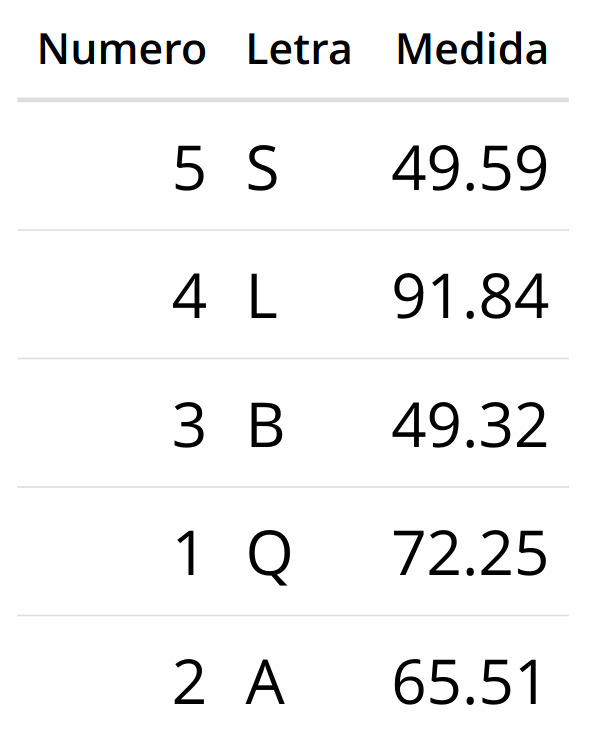
\includegraphics[width=8.33in]{df}

  \bibliography{book.bib,packages.bib}

\end{document}
